\section{Capturing electronic correlation}
\label{sec:Correlation}

\HF is an approximation (albeit a pretty good one)
question is physically what is missed.

\subsection{What does Hartree-Fock miss?}
% Think in terms of SCF procedure

% Averaging approach


\begin{figure}
	\centering
		\begin{tabular}{cc}
		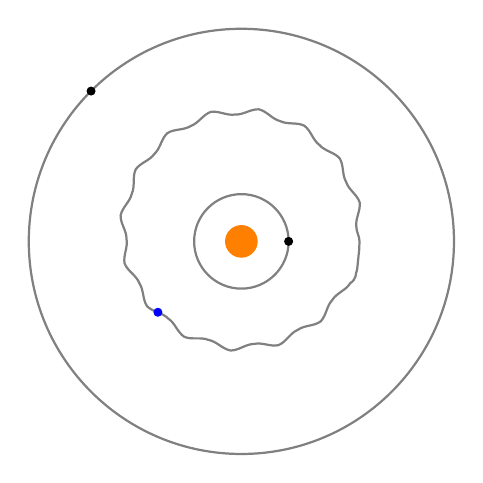
\begin{tikzpicture}[decoration={snake,amplitude=.4mm,segment length=6mm,post length=1mm}]
			\draw [gray,thick,radius=2.7cm] (0,0) circle;
			\draw [gray,decorate,thick,radius=1.5cm] (0,0) circle;
			\draw [gray,thick,radius=0.6cm] (0,0) circle;
			\filldraw [draw=orange,fill=orange,radius=0.2cm] (0,0) circle; 

			\node [shape=circle,draw=black,fill=black,inner sep=1pt] at (0.6,0) {};
			\node [shape=circle,draw=blue,fill=blue,inner sep=1pt] at (-1.060,-0.9) {};
			\node [shape=circle,draw=black,fill=black,inner sep=1pt] at (-1.909,1.909) {};
		\end{tikzpicture}
		&
		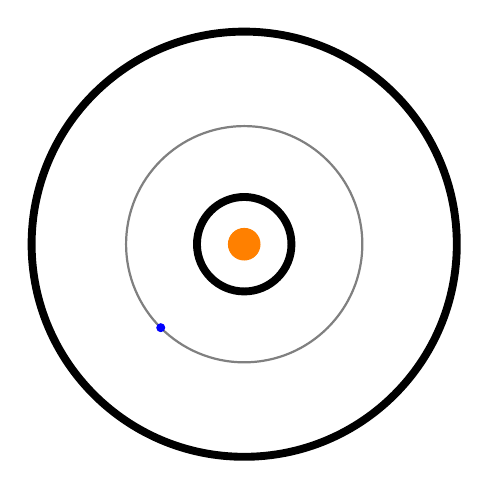
\begin{tikzpicture}[decoration={snake,amplitude=.4mm,segment length=6mm,post length=1mm}]
			\draw [line width=0.1cm,radius=2.7cm] (0,0) circle;
			\draw [gray,thick,radius=1.5cm] (0,0) circle;
			\draw [line width=0.1cm,radius=0.6cm] (0,0) circle;
			\filldraw [draw=orange,fill=orange,radius=0.2cm] (0,0) circle; 

			\node [shape=circle,draw=blue,fill=blue,inner sep=1pt] at (-1.060,-1.060) {};
		\end{tikzpicture} \\
		reales Planetensystem & Hartree-Fock-Planetensystem
		\end{tabular}
	\caption{\HF and real planetary system}
	\label{fig:HFplanets}
\end{figure}


% effective one-particle problem
%	-> show picture of cloud of interactions
%	-> show planetary system picture
% averaged interactions
% show dsa pictures



%still a good ansatz
\begin{itemize}
\item
$\psi$ HF orbitals or (SCF) orbital basis,
typically in FCI one uses the HF orbital basis as the one-particle basis functions for FCI
	\end{itemize}


\todo[inline,caption={}]{
	\begin{itemize}
		\item What is it and where does HF fail
		\item A couple of sentences about truncated CI
			\begin{itemize}
				\item Brief explanation what
				\item Mention size-consistency issues
			\end{itemize}
	\end{itemize}
}

Correlation energy: Difference HF to FCI
(even though HF not fully uncorrelated)

dynamic vs. static correlation


We will discuss so-called \newterm{truncated CI methods},
which only include determinants up to a certain
degree of excitations (double, triple, quadruple, \ldots)
in the context of so-called correlation methods in \vref{sec:Correlation}.


\subsection{Second order Møller-Plesset perturbation theory}
\label{sec:MP}

% reference C. Møller, M. S. Plesset, Phys. Rev. 1934, 46, 618.


Follows Rayleigh-Schrödinger PT
introduce 0-th order and perturbation operator
state RS MP2 energy result
show final expression without derivation
introduce $T_2$ amplitude.

\begin{align*}
	\Op{H}_0 &= \sum_i \Op{F}(i) && \text{Sum of Fock operators} \\
	\Op{V} &= \Op{H} - \Op{H}_0 = \sum_{i<j} \frac{1}{r_{ij}} - \sum_i \Op{V}_H(i) - \sum_i \Op{V}_x(i) && \text{Perturbation operator}
\end{align*}
with
\begin{align*}
	&\Op{F}(i) && \text{Fock operator for electron $i$} \\
	&\Op{V}_H(i) && \text{Hartree potential operator for electron $i$} \\
	&\Op{V}_x(i) && \text{Exchange potential operator for electron $i$} \\
\end{align*}
one gets for the MP2 energy
\begin{align*}
	E_\text{MP2} = \sum_\tau \frac{ \abs{ \bra{\Psi_\text{HF}} \Op{V} \ket{\op{\tau} \Psi_\text{HF}} }^2 }
	{ E_0 - \bra{\Psi_\text{HF}\op{\tau}^\dagger } \Op{H}_0 \op{\tau} \ket{\Psi_\text{HF}}}
\end{align*}
where $\tau$ runs over all possible excitation operators and
\[
	E_0 = \sum_{i \in Occ} \varepsilon_i 
\]

unrestricted
\[ E_\text{MP2} = \frac14 \sum_{\substack{i,j \in Occ \\ a,b \in Virt}}
	\frac{\abs{ \eriMu{ia}{jb} - \eriMu{ja}{ib}}^2 }
	{ \varepsilon_i + \varepsilon_j - \varepsilon_a - \varepsilon_b} \]


\subsection{Coupled-cluster theory}
\defineabbr{CC}{CC\xspace}{Coupled cluster}
\label{sec:CC}

Without going into too many details
the coupled-cluster ansatz generates a wavefuction from the reference
determinant $\Phi_0$ using the exponential ansatz
\[ \Psi_\text{CC} = \exp(\op{T}) \Phi_0 \]
where
\[ \op{T} = \sum_\mu t_\mu \op{\tau}_\mu \]
Variational ansatz leads to full CI.
Instead insert ansatz into electronic Schrödinger equation
\[ \Op{H}_{\Nelec} \exp(\op{T}) \Phi_0 = E_0 \exp(\op{T}) \Phi_0 \]
Introduce similarity-transformed Hamiltonian
\[ \Op{H}_T = \exp(-\op{T}) \Op{H}_{\Nelec} \exp(\op{T}) \]
to write
\begin{align*}
	\mbra{\Phi_0} \Op{H}_T \mket{\Phi_0} &= E \\
	\mbra{\Phi_\mu} \Op{H}_T \mket{\Phi_0} &= 0
\end{align*}
where
\[ \Phi_\mu = \op{\tau} \Phi_0 \]
Projection ansatz not exact.
Number of projections equals number of excitations to consider.

size-extensive and size-consistent treatment

Consider special case of CCD
where $\op{T} = \op{T}_2 = $ doubles only.



$T_2$ amplitudes $t_{ij}^{ab}$
% adapt ccd example of molsturm to this

\defineabbr{CCD}{CCD\xspace}{Coupled cluster doubles}

Working equations
\begin{equation}
\begin{aligned}
	r_{ij}^{ab}
		&= \eriAsym{ab}{ij} \\
		%
		&+ \sum_e f_{ae} \, t_{ij}^{eb}
		 - \sum_e f_{be} \, t_{ij}^{ea}
		 - \sum_m f_{mi} \, t_{mj}^{ab}
		 + \sum_m f_{mj} \, t_{mi}^{ab} \\
		%
		&+ \frac12 \sum_{mn} \eriAsym{mn}{ij} \, t_{mn}^{ab}
		+ \frac12 \sum_{ef} \eriAsym{ab}{ef} \, t_{ij}^{ef} \\
		%
		&+ \sum_{me} \eriAsym{mb}{ej} \, t_{im}^{ae}
		 - \sum_{me} \eriAsym{mb}{ei} \, t_{jm}^{ae} \\
		&- \sum_{me} \eriAsym{ma}{ej} \, t_{im}^{be}
		 + \sum_{me} \eriAsym{ma}{ei} \, t_{jm}^{be} \\
		%
		&- \frac12 \sum_{mnef} \eriAsym{mn}{ef} \, t_{mn}^{af} \, t_{ij}^{eb}
		 + \frac12 \sum_{mnef} \eriAsym{mn}{ef} \, t_{mn}^{bf} \, t_{ij}^{ea} \\
		&- \frac12 \sum_{mnef} \eriAsym{mn}{ef} \, t_{in}^{ef} \, t_{mj}^{ab}
		 + \frac12 \sum_{mnef} \eriAsym{mn}{ef} \, t_{jn}^{ef} \, t_{mi}^{ab} \\
		&+ \frac14 \sum_{mnef} \eriAsym{mn}{ef} \, t_{mn}^{ab} \, t_{ij}^{ef}
		 + \frac12 \sum_{mnef} \eriAsym{mn}{ef} \, t_{im}^{ae} \, t_{jn}^{bf} \\
		&- \frac12 \sum_{mnef} \eriAsym{mn}{ef} \, t_{jm}^{ae} \, t_{in}^{bf}
		 - \frac12 \sum_{mnef} \eriAsym{mn}{ef} \, t_{im}^{be} \, t_{jn}^{af} \\
		&+ \frac12 \sum_{mnef} \eriAsym{mn}{ef} \, t_{jm}^{be} \, t_{in}^{af}
\end{aligned}
	\label{eqn:CCDworking}
\end{equation}
expain terms

see original paper \cite{Bartlett1978}
or detailed derivation \cite{Hodecker2016}


\begin{equation}
	E_\text{CCD} = \frac14 \sum_{ijab} \eriAsym{ij}{ab} t_{ij}^{ab}
	\label{eqn:CCDenergy}
\end{equation}


\defineabbr{ADC}{ADC\xspace}{Algebraic-diagramatic construction}
\subsection{Excited states methods}
Drop names no details
eom-CC
lr-CC
adc
